\documentclass{beamer}

\usepackage{amsfonts}
\usepackage{amsmath}
\usepackage{amsthm}
\usepackage{array}
\usepackage{calc}
\usepackage{framed}
\usepackage{tikz}

\usepackage{xcolor}
\usepackage{ragged2e}

\newtheorem*{claim}{Claim}
\setbeamercolor{claim}{bg = green, fg =black}

\usetikzlibrary{calc}
\usetikzlibrary{positioning, shapes.geometric}
\usetikzlibrary{snakes}


\DeclareMathOperator*{\diam}{diam}
\definecolor{mygold}{rgb}{0.847, 0.702, 0.396}
\definecolor{myblue}{rgb}{0.353, 0.706, 0.675}
\definecolor{DarkGreen}{rgb}{0.0, 0.5, 0.0} % Adjust values for a darker shade


%macro for problem boxes
\newcommand{\prob}[1]{\textnormal{\textsc{#1}}\xspace}

% Problem environment
\newenvironment{tightcenter}
	{\parskip=0pt\par\nopagebreak\centering}
	{\par\noindent\ignorespacesafterend}

\let\tnote\relax

\newlength{\RoundedBoxWidth}
\newsavebox{\GrayRoundedBox}
\newenvironment{GrayBox}[1]%
{\setlength{\RoundedBoxWidth}{\linewidth-4.5ex}
\def\boxheading{#1}
\begin{lrbox}{\GrayRoundedBox}
\begin{minipage}{\RoundedBoxWidth}%
}{%
\end{minipage}
\end{lrbox}%
\begin{tightcenter}%

\begin{tikzpicture}%
\node(Text)[draw=black!20,fill=white,rounded corners,%
inner sep=2ex,text width=\RoundedBoxWidth]%
{\usebox{\GrayRoundedBox}};
\coordinate(x) at (current bounding box.north west);
\node [draw=white,rectangle,inner sep=3pt,anchor=north west,fill=white]
at ($(x)+(10.5pt,.75em)$) {\boxheading};
\end{tikzpicture}
\end{tightcenter}\vspace{0pt}%
\ignorespacesafterend}

\newenvironment{problembox}[1]{\noindent\ignorespaces%
\FrameSep=6pt%
\parindent=0pt%
\vspace*{-.5em}
\begin{GrayBox}{\textsc{#1}}%
\newcommand\Input{Input:}%
\newcommand\Prob{Problem:}%
\begin{tabular*}
    {\columnwidth}
    {@{\hspace{-0.5em}} >{\itshape} p{4.8em} p{0.8\columnwidth} @{}}
}{
\end{tabular*}%
\end{GrayBox}%
\vspace*{-1.0em}
\ignorespacesafterend}
%end macro declaration




\usetheme{Madrid}
\usecolortheme{default}



\title{Maximizing the Guarded Boundary of a Dynamic Art Gallery}
\author{Mihir Patel}


\begin{document}

\frame{\titlepage}


\begin{frame}
  \frametitle{Art Gallery}
  \centering
  \begin{center}
      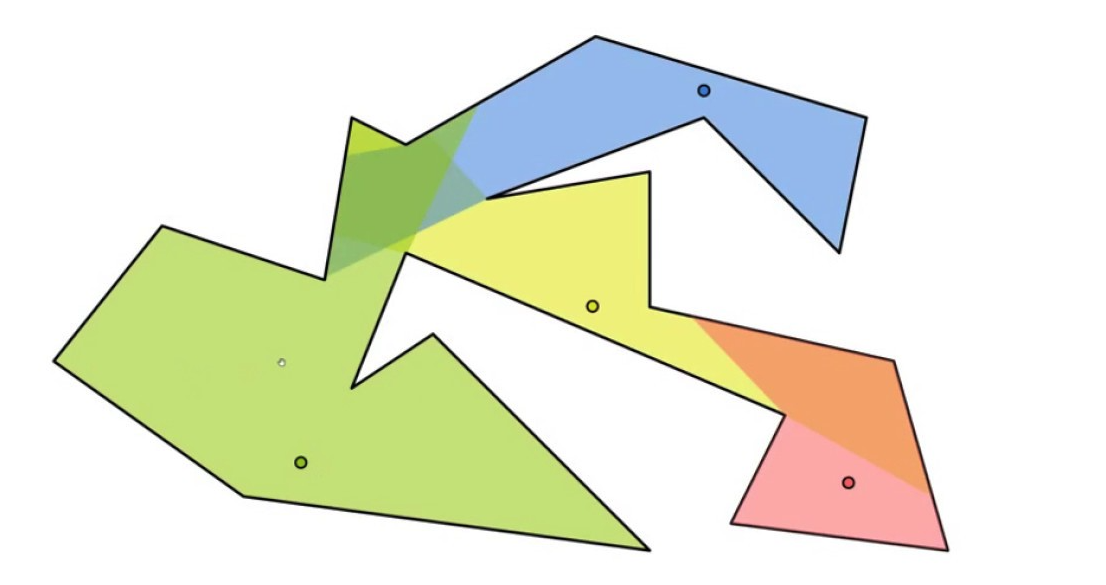
\includegraphics[width=0.8\textwidth]{figures/art-gallery.png}
      \vspace{1em}
  \end{center}
  \textcolor{DarkGreen}{\textbf{Problem:}} Given a polygon $P$, find the minimum number of guards needed to guard the whole polygon.
\end{frame}

\begin{frame}
    \centering
    \frametitle{Flipping what we optimize}
    \begin{center}
      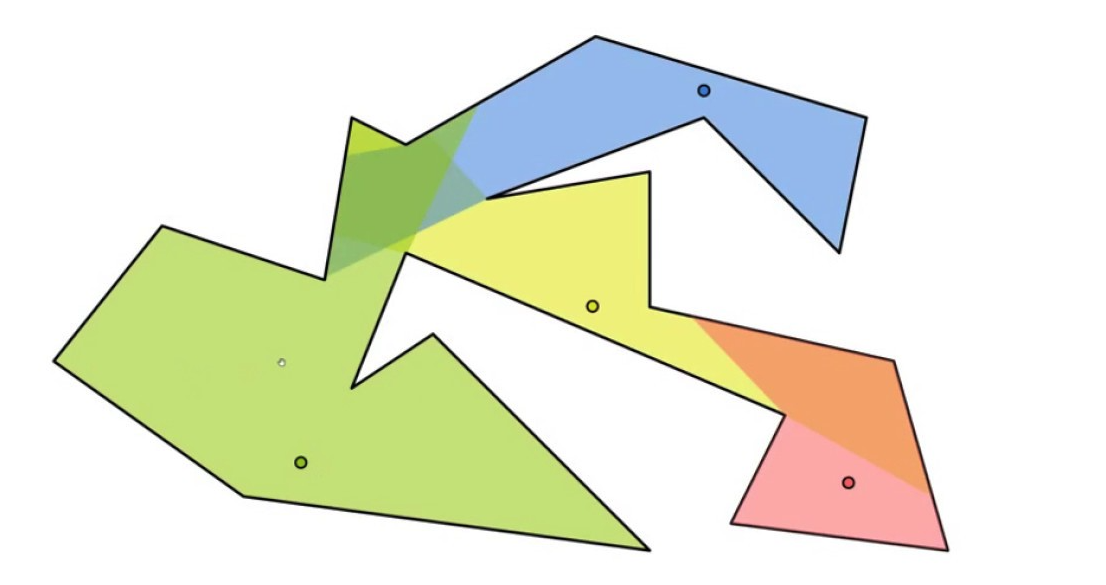
\includegraphics[width=0.8\textwidth]{figures/art-gallery.png}
      \vspace{1em}
    \end{center}
    \only<1>{
        \textcolor{DarkGreen}{\textbf{Problem:}} Given a polygon $P$ and $k\in\mathbb{N}$, find the maximum area that can be guarded by $k$ guards.
    }
    \only<2>{
        \textcolor{DarkGreen}{\textbf{Problem:}} Given a polygon $P$ and $k\in\mathbb{N}$, find the maximum area that can be guarded by $k$ \textcolor{red}{vertex} guards.
    }
    \only<3>{
        \textcolor{DarkGreen}{\textbf{Problem:}} Given a polygon $P$ and $k\in\mathbb{N}$, find the maximum \textcolor{red}{boundary length} that can be guarded by $k$ \textcolor{red}{vertex} guards.
    }
\end{frame}

\begin{frame}
    \frametitle{A weighted case}
    \emph{Some paintings are more valuable than others, and with limited guards they should be of greater concern.}\\\pause
    \begin{center}
      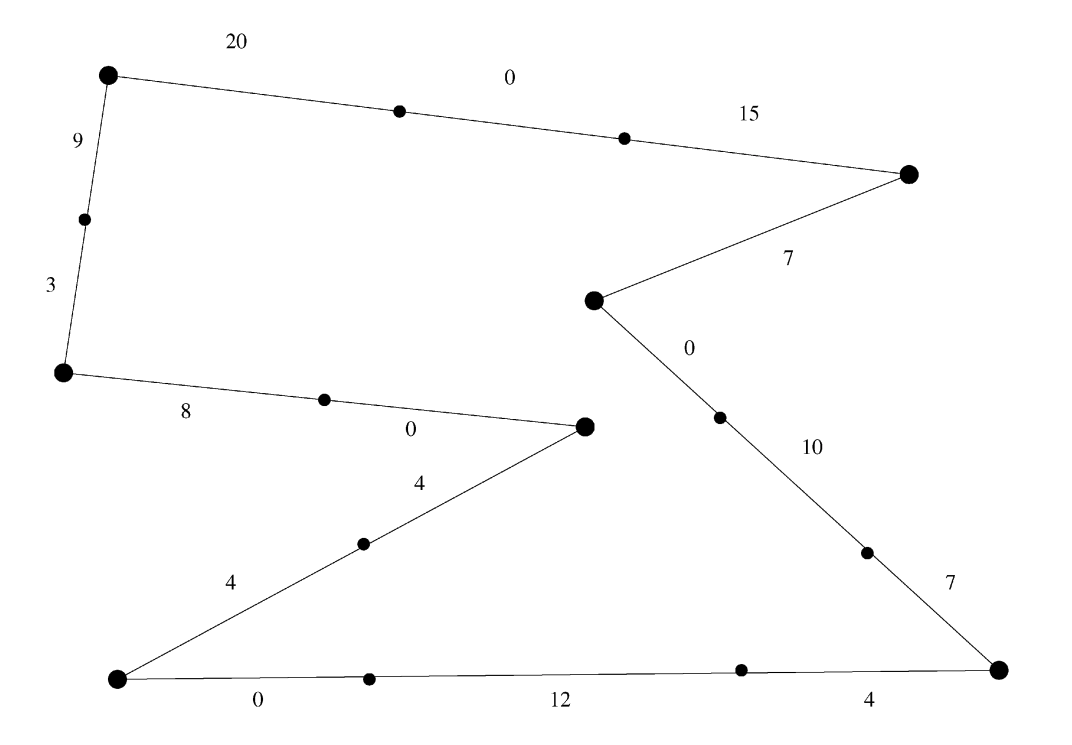
\includegraphics[width=8cm]{figures/weighted-polygon.png}
    \end{center}\pause
    \textcolor{DarkGreen}{\textbf{Problem:}} Given a polygon $P$ and $k\in\mathbb{N}$, find the maximum value that can be guarded by $k$ vertex guards.
\end{frame}

\begin{frame}
  \frametitle{Existing Results}
  Fragoudakis et. al (2005,2006,2007)\\
  \begin{problembox}{Maximum Length Vertex Guard}
    \Input& A simple polygon $P$ and positive integer $k\in\mathbb{N}$. \\
    \Prob& Find a set of vertices $S\subseteq V_P$ of size at most $k$ such that \textcolor{red}{$L(S)$} is maximized. \\
  \end{problembox}\\\pause

  \begin{problembox}{Maximum Value Vertex Guard}
    \Input& A simple polygon $P$ and positive integer $k\in\mathbb{N}$. \\
    \Prob& Find a set of vertices $S\subseteq V_P$ of size at most $k$ such that \textcolor{red}{$W(S)$} is maximized. \\
  \end{problembox}\pause
  Both problems are APX-complete and permit $(1-1/e)$-approximations. 
\end{frame}

\begin{frame}
  \frametitle{Proposed Contributions}
  \begin{itemize}
    \item Improving simplicity (and possibly runtime) of current results for unweighted/weighted case.\pause
    \item Difficult to break past monotone/submodular $\rightarrow$ hardness of approximation results?
  \end{itemize}
\end{frame}

\begin{frame}
  \frametitle{Set Cover}
  \centering
  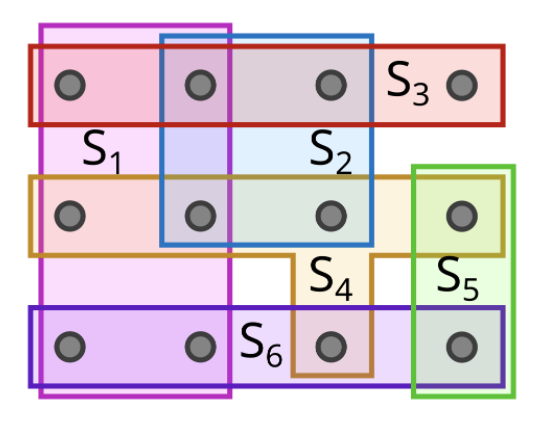
\includegraphics[width=6cm]{figures/set-cover.png} % Replace
  \begin{problembox}{Set Cover}
    \Input& A universe $U$ of $n$ elements, $m$ subsets of $U$. \\
    \Prob& What is the \textcolor{red}{minimum number of subsets} whose union covers all of $U$? \\
  \end{problembox}
  
\end{frame}


\begin{frame}
  \frametitle{Max Coverage}
  \centering
  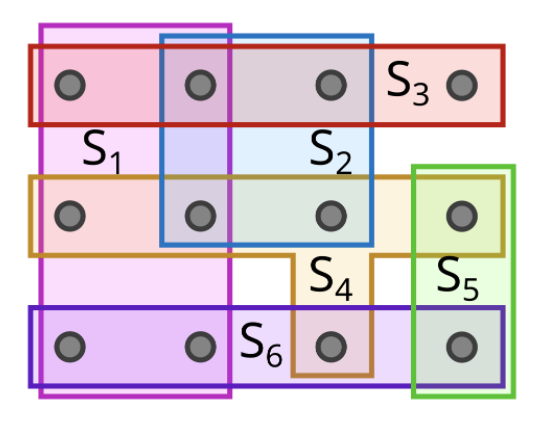
\includegraphics[width=6cm]{figures/set-cover.png} % Replace
  \begin{problembox}{Max Coverage}
    \Input& A universe $U$ of $n$ elements, $m$ subsets of $U$, $k\in\mathbb{N}$. \\
    \Prob& What is the \textcolor{red}{maximum number of elements} in $U$ covered by the union of $k$ subsets? \\
  \end{problembox}
\end{frame}

% \begin{frame}
%   \frametitle{Monotonicity and Submodularity}

%   \begin{itemize}
%     \item \textbf{Monotonicity:} \\
%       For any sets $S \subseteq T$, we have:
%       \[
%         f(S) \leq f(T)
%       \]
%     \pause
%     \item \textbf{Submodularity:} \\
%       For any sets $S \subseteq T$ and element $x \notin T$, we have:
%       \[
%         f(T \cup \{x\}) - f(T) \leq f(S \cup \{x\}) - f(S)
%       \]
%   \end{itemize}\pause

%   \vspace{0.5em}

%   \begin{theorem}
%     Greedily maximizing a monotone, submodular objective function achieves a $(1 - 1/e)$-approximation to the optimal value.
%   \end{theorem}\pause

%   \vspace{0.5em}

%   \textbf{Example:} Max Coverage
% \end{frame}





\begin{frame}
    \frametitle{A dynamic version}
    Paintings may move around, new paintings may arrive. You need to find an optimal camera placement that does not require extensive reinstallment.\\\pause
    \centering
    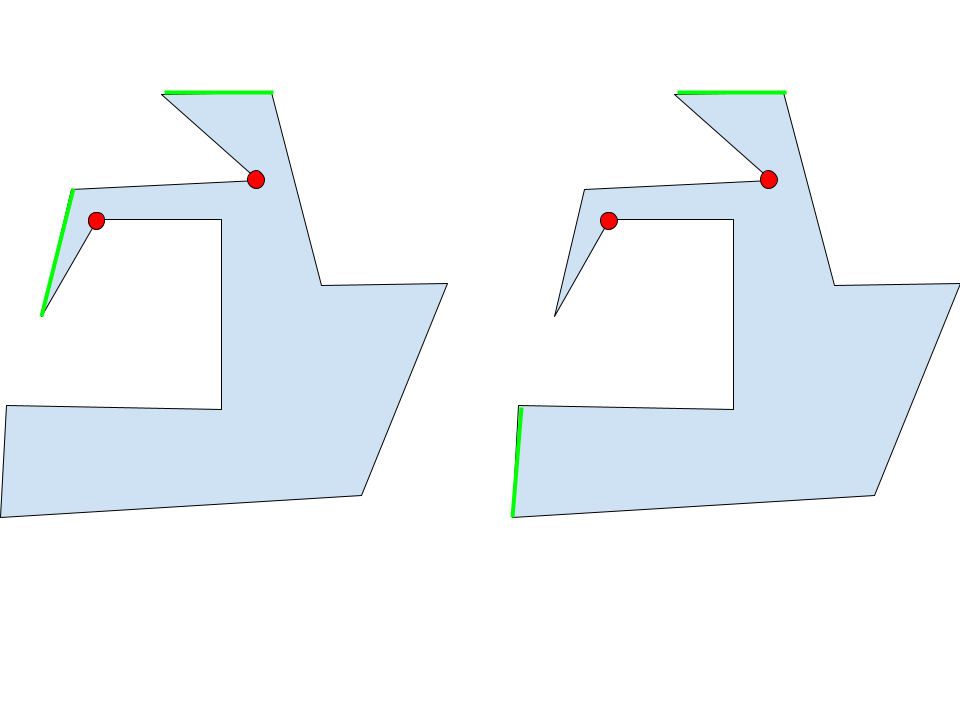
\includegraphics[width=12cm]{figures/dynamic-gallery.png} % Replace
\end{frame}





\begin{frame}
  \title{Thank You!}
  \begin{center}
      \Huge{\textbf{Thank You!}} \\
      \vspace{1em}
      \Large{\textit{Questions?}} \\
      \vspace{2em}
  \end{center}
\end{frame}

\end{document}



